\begin{frame}{Дополнительный слайд 1. Тёмный солитон}
	\vfill
	
	% --- ВЕРХНИЙ ЯРУС: МАТЕМАТИЧЕСКАЯ ПОСТАНОВКА ---
	\begin{columns}[T]
		\begin{column}{0.49\textwidth}
			\begin{tcolorbox}[
				colframe=DeepBlue!35, 
				colback=DeepBlue!1!Ivory, 
				coltext=DeepBlue, 
				boxrule=0.5pt, arc=3pt, 
				top=4pt, bottom=4pt, left=5pt, right=5pt,
				before=\vspace{0pt}, after=\vspace{0pt},
				equal height group=nls_math
				]
				\scriptsize
				$$\mathbf{i u_t + u_{xx} + u_{yy} - |u|^2 u + u = 0}$$
				$$\mathbf{u(x, y, t) = \sqrt{2} \tanh(x - 2t) e^{i(x - 2t)}}$$
			\end{tcolorbox}
		\end{column}
		
		\begin{column}{0.49\textwidth}
			\begin{tcolorbox}[
				colframe=Burgundy!35, 
				colback=Burgundy!1!Ivory, 
				coltext=DeepBlue, 
				boxrule=0.5pt, arc=3pt, 
				top=4pt, bottom=4pt, left=5pt, right=5pt,
				before=\vspace{0pt}, after=\vspace{0pt},
				equal height group=nls_math
				]
				\scriptsize
				$$\mathbf{|u(x, y, t)|^2 = 2 \tanh^2(x - 2t)}$$
				$$\mathbf{M[u](t) = \int_{\Omega} |u(x, y, t)|^2 dx dy \equiv \text{const}}$$
			\end{tcolorbox}
		\end{column}
	\end{columns}
	
	\vspace{0.3cm}
	
	% --- НИЖНИЙ ЯРУС: ГРАФИКИ (КАРТИНКИ) ---
	\begin{columns}[T]
		
		% Левый график — динамика интенсивности
		\begin{column}{0.49\textwidth}
			\centering
			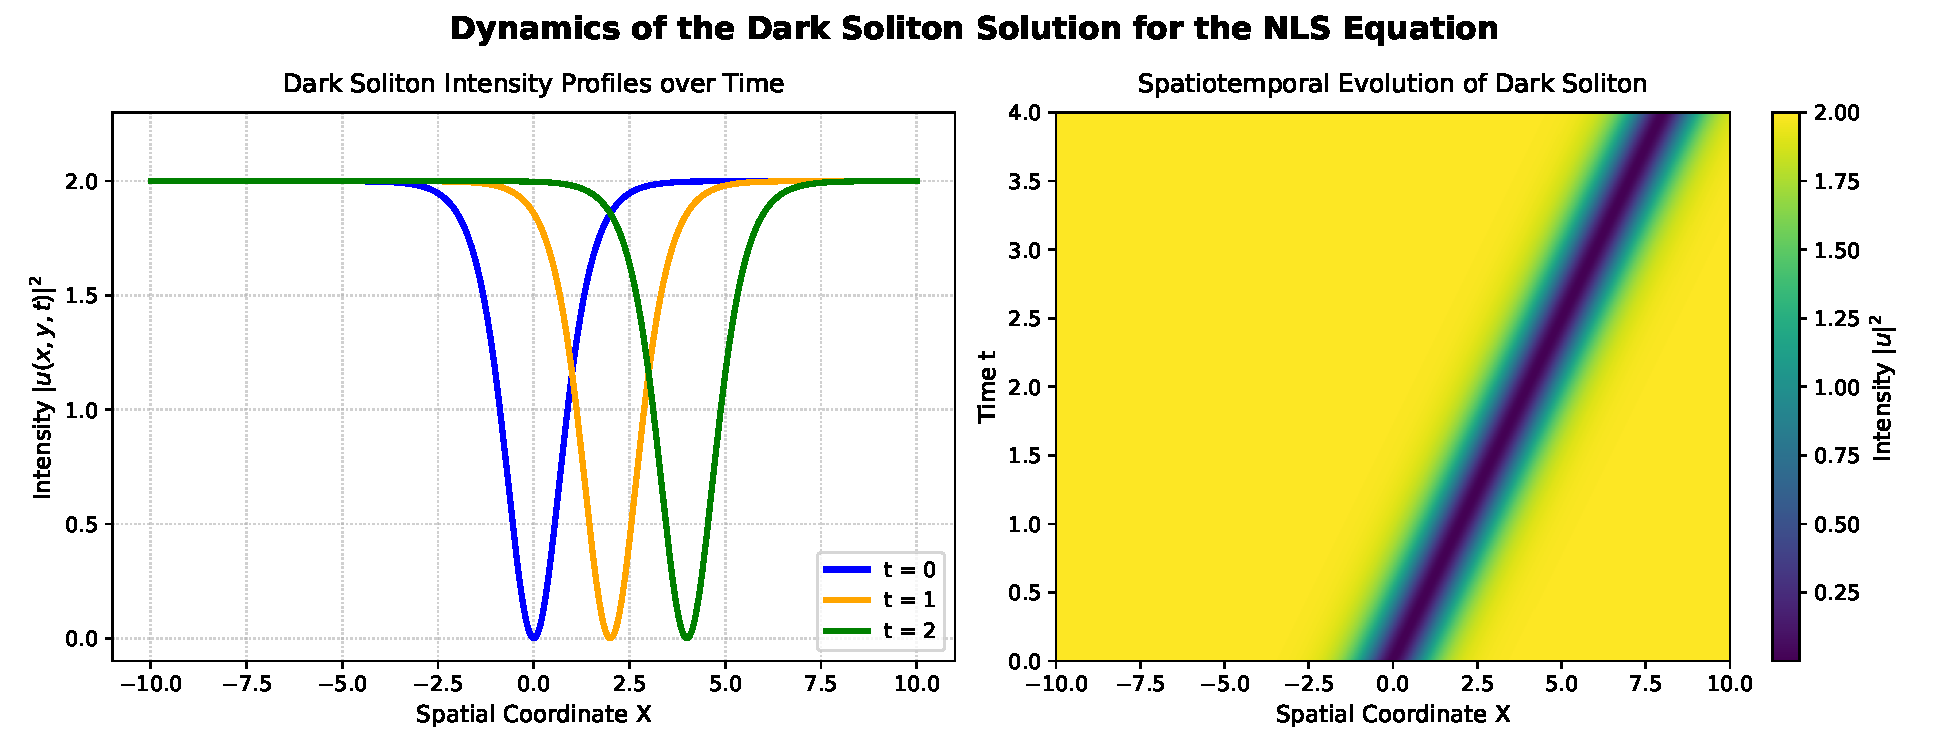
\includegraphics[width=0.95\linewidth]{../illustrations/results/dark_soliton_dynamics}
		\end{column}
		
		% Правый график — осцилляции компонент
		\begin{column}{0.49\textwidth}
			\centering
			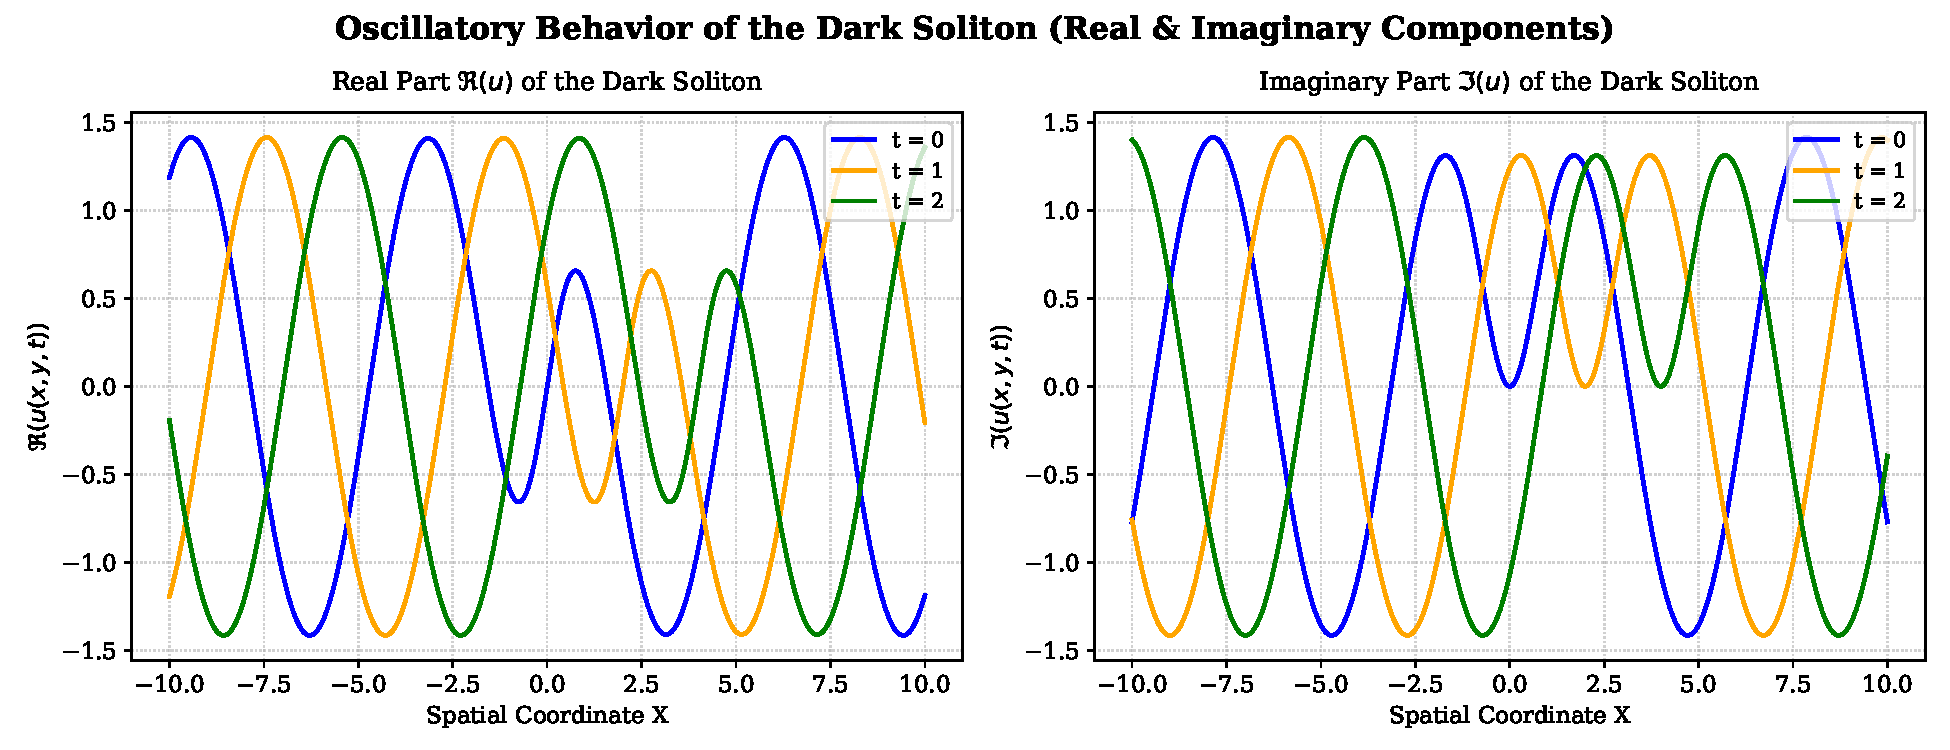
\includegraphics[width=0.95\linewidth]{../illustrations/results/dark_soliton_real_imag}
		\end{column}
		
	\end{columns}
	
	\vfill
\end{frame}